%!TEX root = ../main.tex

\chapter {Theoretical Foundation}
\label {cha:theoretical foundation}
% Einleitung schreiben

\section{Definitions}
\label{sec:definitions}

The definition of unreachable code is rather complicated and confusing. 
Similar terms like dead code and infeasible code are often tossed around and the definition appears to differ in many standards. 
Sometimes the terms are used as aliases for each other.


In the following Sections, each term will be defined.

\subsection{Unreachable code}
\label{sub:unreachable code}
unreachable code is source code, which can never be reached (during execution). 
The causes may either be due to:
\begin{enumerate}
	\item Imperative statements that force an unconditional jump (even though there are statements following) as shown in Listing \ref{code:unconditional unreachable code}. Depending on language, these statements are 
	\begin{itemize}
		\item break
		\item return
		\item goto
	\end{itemize}
	\item infeasible conditions as described in section \ref{sub:infeasible code}. 
\end{enumerate}


\begin{program}[h!]
	\begin{CppCode}
		int unreachable_code_goto() {
			int x = 42;
			goto end;
			x = 43; // unreachable
			end: return x;
		}
		
		int unreachable_code_return() {
			int x = 42;
			return x;
			x = 43; // unreachable
		}
		
		int unreachable_code_break() {
			int x = 42;
			while(true) {
				break;
				x = 43; // unreachable
			}
			return x;
		}
		
		int unreachable_code_exception(int x) {
			if(x != 42) {
				throw "X is not 42";
				x = 42; // unreachable
			}
			return x;
		}
		
		int checked_conditions(int x) {
			if(x == 42) {
				return 42;
			} else if(x == 42) { // This condtion was checked already => unreachable
				return 42;
			}
			return x;
	}\end{CppCode}
	\caption{This example written in C++ demonstrates unreachable code due to unconditional jumps. When conditions were already checked within the same if-then-else block they are also considered unreachable.}
	\label{code:unconditional unreachable code}
\end{program}


\subsection{Dead Code}
\label{sub:dead code}

Dead code is code, which may be reachable, but is not used any further.
The most common types of dead code is unused code:
\begin{itemize}
	\item Unused variables \cite{Prahofer_2012}
	\item Unused methods/functions \cite{Romano_2016}
	\item Unused classes
	\item Unused files \cite{Boomsma_2012}
	\item ...
\end{itemize}
In Listing \ref{code:dead code} some of these errors are presented. As presented, unnecessary assignments are also considered dead code.


The term \emph{dead} implies that the counterpart called \emph{live} exists. 
The \emph{Liveness} of an expression indicates if it has any impact on the program when executed.
Dead code is usually a sign of an unnecessary baggage and should be deleted, which is often easy since it is not used anyways.
When dead code is not deleted and more and more instances of dead code are accumulated, it will become harder to maintain and comprehend \cite{Romano_2020}. Dead code may be intended in foresight of extensibility. But when this extensibility is no longer intended, the already implemented mechanisms may include dead code. This code must be refactored or removed, otherwise it results in worse maintainability and 
source code written in object-oriented programming languages do contain significantly more dead code according to the research paper \cite{Srivastava_1992}.


It is important to note that according to this definition dead code may be reachable, but does not have to be.

% \cite{Romano_2016}
% \cite{Boomsma_2012}

% Unused statements, methods, variables (?)

\begin{program}[h!]
	\begin{JavaCode}
		public class DeadCode {
			public static int unusedVariable() {
				int i = 1; // Unused variable
				int j = 3;
				int x = 3 + j;
				return x;
			}
			
			public static int unnecessaryAssignment() {
				int x;
				x = 4; // Unnecessary Assignment
				x = 3;
				return x;
			}
			
			private static class UnusedClass {
				// This class is not used (and cannot be accessed from outside this class)
			}
			
			private static void unusedMethod() {
				// This method is not used (and cannot be accessed from outside this class)
			}
	}\end{JavaCode}
	\caption{Some instances of dead code written in Java. The unnecessary assignment in line 11 does not have any effect. In case the file containing the class DeadCode is not used it would be considered as a dead file.}
	\label{code:dead code}
\end{program}

\subsubsection{Is Unreachable Code Dead Code?}
% Pro / Contra
Dead code and unreachable code are often used synonymously. 
Some standards, like MITRE-CWE \cite{CWECWE561Dead} define dead code as follows:
\begin{quote}
	Dead code is source code that can never be executed in a running program. The surrounding code makes it impossible for a section of code to ever be executed.
\end{quote}
This definition does not have anything in common with the one provided before. According to this standard, dead code is unreachable code, since it cannot be executed. But unnecessary assignments are not considered dead code, but has its own category \emph{Assignment to Variable Without Use}.
Both of these issues are considered as \emph{Irrelevant Code}.

\pagebreak
In contrast the standard MISRA-C \cite{motorindustrysoftwarereliabilityassociationMISRAC2004Guidelines2008} defines unreachable code as follows:
\begin{quote}
	Rule 14.1 (required): There shall be no unreachable code.
	This  rule  refers  to  code,  which  cannot  under  any  circumstances  be  reached,  and  which  can  be 
	identified at compile time. Code that can be reached but may never be executed is excluded 
	from the rule (e.g., defensive programming code).	
\end{quote}
Semantically both definitions are the same. The only difference is the naming.


The similarity between unreachable code and dead code is that both do not have an effect on a running program. But dead code (as described in this document) may be reachable, but is just unnecessary, especially when executed. 


As mentioned before the sources of these two error types are different.
Dead code occurs for example, when intended extensibility or features are no longer required and are not deleted or refactored.
Unreachable code, especially infeasible code, occurs due to faulty logic and may not as straightforward to fix.
\subsection{Infeasible Code}
\label{sub:infeasible code}
Infeasible code is a subset of unreachable code.
Infeasible code only occurs due to conditions which always evaluate to false. Another reason could be confusion around expressions \cite{Eichberg_2015}.


Infeasible code may occur either due to conditions which only consist of boolean literals (and expressions), constants, or as consequence of former conditions, as demonstrated in Listing \ref{code:infeasible code}.


\begin{program}[h!]
	\begin{JavaCode}
		public class InfeasibleCode {
			public static void infeasibleConstant() {
				if(false) {
					// always false
					// ...
				}
			}
			
			public static void alwaysInfeasibleVariable() {
				boolean x = false;
				if(x) {
					// always false
					// ...
				}
			}
			
			public static void infeasibleConditions(int x) {
				if(x > 10) {
					if(x < 10) {
						// always false
						// ...
					}
				}
			}
	}\end{JavaCode}
	\caption{Infeasible code is determined by conditions which always result with false. }
	\label{code:infeasible code}
\end{program}

\section{IEC 61131-3}
\label{sec:iec}

IEC 61131-3 is a standard, which concern the programming of PLCs (\emph{Programmable Logic Controller}). The standard does not describe itself as a rigid set of rules, but rather a guideline \cite{johnIEC611313Programming2010}. The implementation of this standard requires at least some features, but not necessarily all. Manufactures must declare, which requirements were implemented. This is done by feature tables, which are included in the standard. Benchmarks for assessing how close an implementation adheres to a standard are also included.


The standard is maintained by the independent organization PLCOpen \cite{eldijkWhatPLCopen2018}, which was founded in 1992 (after IEC 61131-3 was published) with a manufacturer and product independent standard in mind.


The standard does not only provide guidelines for manufacturers, but also for projects of end users \cite{johnIEC611313Programming2010}.
\pagebreak
\subsection{Program Organization Unit (POU)}
\label{sub:pou}
Projects are built of POUs. These organization units are encapsulated, which does not only modularize code, but also enables independent compilation.
There are three types of POUs \cite{johnIEC611313Programming2010}:
\begin{itemize}
	\item \emph{FBs} (\emph{Functionblock}) are the main building blocks of a program. Function blocks can be instantiated. They may contain actual state (like a timer or counter). Function block types are visibly globally, but instances may not be. Inheritance is not intended.
	\item \emph{Programs} represent the main program. These units are not called explicitly by other POUs, but otherwise behave like FBs.
	\item \emph{Functions} basically are the same as regular, pure functions. Therefore functions do not contain any state and are not able to call Function Blocks, which may contain side effects. 
\end{itemize}
POUs contain two parts:
\begin{itemize}
	\item \emph{Declaration} of variables. Every variable that is used must be declared before. Elementary data types are booleans, signed and unsigned integers, reals, time, dates, durations and strings. Furthermore programmers may define their own custom datatypes using type definitions, enumerations and arrays.
	\item \emph{Code} which contains the logic written in one of the languages mentioned in Section \ref{sub:iec-lang}.
\end{itemize}
POUs can be called with or without parameters. Parameters may be provided directly or via global/external variables.

Recursion is not allowed, neither directly nor indirectly. 


\subsection{Languages}
\label{sub:iec-lang}
The logic part of POUs may be implemented in one of five distinct programming languages \cite{johnIEC611313Programming2010}:
\begin{itemize}
	\item \emph{Instruction List} is an assembly like programming language (see Listing \ref{code:il}). Other languages are translated into this language.
	\item \emph{Structured Text} is described in Section \ref{sub:structured text}.
	\item \emph{Function block Diagram} are partly graphical and partly textual (see Figure \ref{code:fbd}). The language is inspired from the field of signal processing. 
	\item \emph{Ladder Diagram} is a graphical language, mainly used when processing boolean values (see Figure \ref{code:ld}).
	\item \emph{Sequential Function Chart} is a graphical language, whose goal is to break complex programs into small manageable units (see Figure \ref{code:sfc}). 
\end{itemize}

\begin{program}[h!]
	\begin{GenericCode}
VAR
	FirstOperand, SecondOperand, Result: INT := 10;
	StringOp: String[30] := '12345678901234567890';
	StringRes: String[25];
END_VAR
		
B1:	LD FirstOperand (* 10 {INT} *)
ADD SecondOperand (* 20 {INT} *)
ST Result (* 20 {INT} *)
GT 0 (* TRUE, because 20 > 0 {BOOL} *)
JMPC B2
(* jump, because CR=TRUE; present value of CR remains {BOOL} *)
JMP FarAway (* CR is not defined or present value: *)
(* implementation-dependent *)
B2: LD StringOp (* 12345678901234567890 {STRING} *)
ST StringRes (* 12345678901234567890 {STRING} *)\end{GenericCode}
	% TODO
	\caption{Example Instruction List program from the book \cite{johnIEC611313Programming2010}.}
	\label{code:il}
\end{program}

%\begin{program}[h!]
%	\begin{GenericCode}
%		TYPE MulVar: STRUCT Var1: INT; Var2: REAL; END_STRUCT; END_TYPE
%		VAR d: INT;
%		e: ARRAY [0..9] OF INT; 
%		f: REAL;
%		g: MulVar (Var1:=10, Var2 := 2.3); 
%		h: MulVar;
%		END_VAR
%		d := 10; (* Assignment *)
%		e[0] := d ** 2;   h  := g; (* Two assignments in one line *)
%		d := REAL_TO_INT(f); (* Assignment evaluating a function call *)\end{GenericCode}
	% TODO
%	\caption{Example structured text program from the book \cite{johnIEC611313Programming2010}.}
%	\label{code:st}
%\end{program}

\begin{figure}[h!]
	\centering
	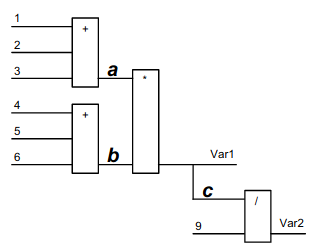
\includegraphics[width=0.7\textwidth]{fbd}
	% TODO
	\caption{Example function block diagram program from the book \cite{johnIEC611313Programming2010}.}
	\label{code:fbd}
\end{figure}

\begin{figure}[h!]
	\centering
	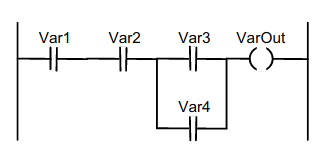
\includegraphics[width=0.5\textwidth]{ld}
	% TODO
	\caption{Example ladder diagram program from the book \cite{johnIEC611313Programming2010}.}
	\label{code:ld}
\end{figure}

\begin{figure}[h!]
	\centering
	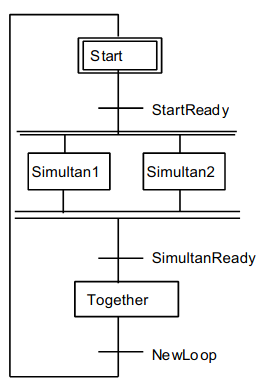
\includegraphics[width=0.4\textwidth]{sfc}
	% TODO
	\caption{Example sequential function chart diagram program from the book \cite{johnIEC611313Programming2010}.}
	\label{code:sfc}
\end{figure}


\subsection{Structured Text}
\label{sub:structured text}
Structured Text is a Pascal-like, high level programming language.
Structured Text programs consist of a number of statements. In comparison to the textual Instruction List language, instructions are separated by semicolons. 
%% TODO vllt im impl kapitel erwähnen
% The implementation mentioned in Chapter \ref{cha:finding unreachable code using a smt-solver} focuses on Structured Text.
In comparison to the Instruction List language, instructions are separated by semicolons. Comments can be written to the end of the line using double slashes. Furthermore there is the possibility for multiline comments which start with an opening parenthesis and an asterisk and end with an asterisk and a closing parenthesis.

Table \ref{tab:st-statements} illustrates all Structured Text statements. Even though no \emph{goto} statement exists in the standard, it may be implemented by vendors. 

% Please add the following required packages to your document preamble:
% \usepackage{graphicx}

\begin{table}[h!]
	%\resizebox{\textwidth}{!}{%
		\begin{tabular}{|l|l|l|L|}
			\hline
			Keyword &
			Description &
			Example &
			Explanation \\ \hline
			:= &
			Assignment &
			d := 10; &
			Assignment of a calculated value on the right to the identifier on the left \\ \hline
			&
			Call of an FB &
			\begin{tabular}[c]{@{}l@{}}FBName(\\   Par1:=10,\\   Par2:=20,\\   Par3:=\textgreater{}Res);\end{tabular} &
			Call of another POU of type FB including its parameters. “:=” for input parameters, “=\textgreater{}” for output parameters \\ \hline
			RETURN &
			Return &
			RETURN; &
			Leave the current POU and return to the calling POU \\ \hline
			IF &
			Selection &
			\begin{tabular}[c]{@{}l@{}}IF d \textless e THEN f:=1;\\ ELSIF d=e THEN f:=2;\\ ELSE f:= 3;\\ END\_IF;\end{tabular} &
			Selection of alternatives by means of Boolean expressions. \\ \hline
			CASE &
			Multi-selection &
			\begin{tabular}[c]{@{}l@{}}CASE f OF\\   1: g:=11;\\   2: g:=12;\\ ELSE g:=FunName();\\ END\_CASE;\end{tabular} &
			Selection of a statement block, depending on the value of the expression "f". \\ \hline
			FOR &
			Iteration (1) &
			\begin{tabular}[c]{@{}l@{}}FOR h:=1 TO 10 BY 2 DO\\   f{[}h/2{]} := h;\\ END\_FOR;\end{tabular} &
			Multiple loop of a statement block with a start and end condition and an increment value. \\ \hline
			WHILE &
			Iteration (2) &
			\begin{tabular}[c]{@{}l@{}}WHILE m \textgreater 1 DO\\   n := n / 2;\\ END\_WHILE;\end{tabular} &
			Multiple loop of a statement block with end condition at the beginning. \\ \hline
			REPEAT &
			Iteration (3) &
			\begin{tabular}[c]{@{}l@{}}REPEAT\\   i := i*j;\\ UNTIL i \textless 10000\\ END\_REPEAT;\end{tabular} &
			Multiple loop of a statement block with end condition at the end. \\ \hline
			EXIT &
			End of loop &
			EXIT; &
			Premature termination of an iteration statement \\ \hline
			; &
			Dummy statement &
			;; &
			\\ \hline
		\end{tabular}%
%	}
% Richtig zitiert?
	\caption{All statements defined by the IEC-61131 standard \cite{johnIEC611313Programming2010}. }
	\label{tab:st-statements}
\end{table}

% Expressions ?

\clearpage
\pagebreak

% TODO
% \section{Static Code Analysis}
% Static code analysis is used to analyze source code for a wide range of different code smells without actually executing the code. 
% The goal is to detect potential errors early as well as hinting to problematic code, which either is too complex or contains unwanted constructs potentially causing errors. 
% Many

% TODO 
%\subsection{Abstract Syntax Tree}
\section{Abstract Syntax Tree}
\label{sub:ast}
Abstract syntax trees (AST) are a hierarchical representation of the abstract syntactic structure of text written in a formal language. The AST is created during parsing and a central piece of compilers and static code analysis tools (described in the introduction of Chapter \ref{cha:state of the art}). This representation does only contain relevant expressions, stripping unnecessary delimiters (e.g., braces). Each node represents an operator, while the children represent the operands as described by Aho \cite{ahoCompilersPrinciplesTechniques2007}. Therefore not only expressions, but whole projects may be represented by a single AST.

As described by Prähofer \cite{Prahofer_2012}, the AST representation of an IEC program begins with the root node of an IEC project, which consists of multiple functional units, their descendants consist of functions and function blocks, which contain IEC code. Therefore all program elements are presented in form of an AST node as shown in Figure \ref{fig:ast basics}.

\begin{figure}[h!]
	\centering
	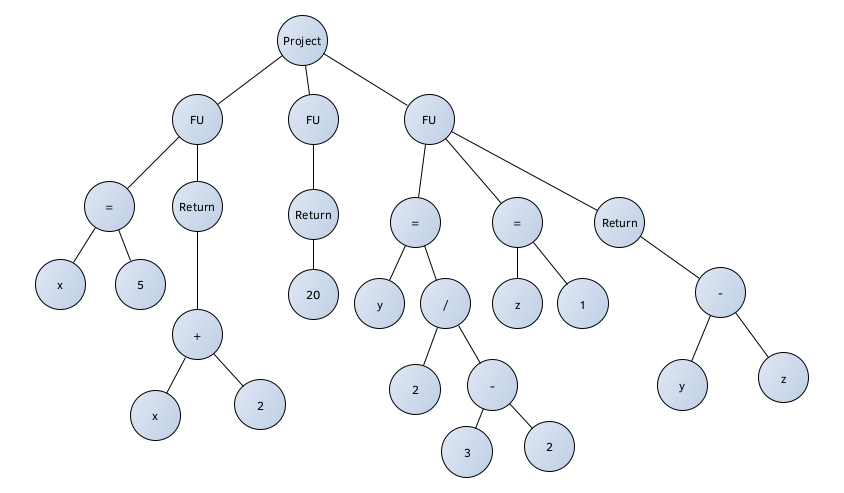
\includegraphics[width=0.9\textwidth]{ast-iec}
	\caption{Example IEC project containing FUs with arithmetic expressions and assignments represented in a simplified AST.}
	\label{fig:ast basics}
\end{figure}

%\subsection{Control Flow Graph}
\section{Control Flow Graph}
\label{sub:cfg}
Control flow graph (CFG) is a form of representation of a program, representing possible paths a program can take. These paths are a result of if-then-else conditions and loops, which also contain conditions, which have to be checked. 
This representation is necessary for certain types of analysis, e.g. dead code analysis or unreachable code analysis.

The control flow graph consists of so called basicblocks, which contains the longest sequence of instructions without any jumps \cite{Prahofer_2012}. Jumps may be conditional (e.g., if-then-else, loops) or unconditional (e.g., break, goto) and are represented by (directed) edges. These edges connect basicblocks (see Figure \ref{fig:cfg basics}). Code without loops represented in form of a CFG contains edges pointing in one direction. Loops may easily be spotted, since they contain an edge to a former block. Basicblocks containing instructions that perform a conditional jumps have two outgoing edges. The first edge contains the path, if the condition evaluates true, the second otherwise. 

Usually a CFG is created for each individual procedure/function. 

\begin{figure}[h!]
	\centering
	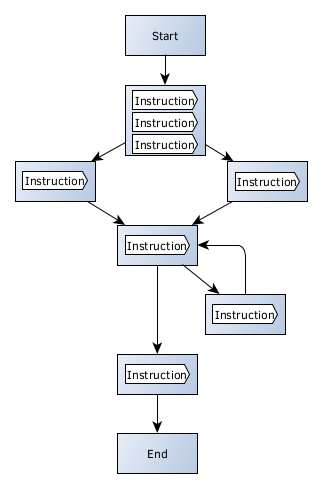
\includegraphics[width=0.5\textwidth]{cfg}
	\caption{Control flow graph of a program consisting of one conditional jump using if-else and another conditional jump for a loop on the right side having an outgoing edge back to a previous basicblock.}
	\label{fig:cfg basics}
\end{figure}

% TODO Subsection über KEMRO-IEC ? oder in IMPL erwähnen... --> In Impl erwähnen

\section{Satisfiable Modulo Theory}

Satisfiable modulo theory (short SMT) is defined as stated in \cite{demouraZ3EfficientSMT2008}:

\begin{quote}
	Satisfiability modulo theories (SMT) generalizes boolean satisfiability (SAT) by
	adding equality reasoning, arithmetic, fixed-size bit vectors, arrays, quantifiers,
	and other useful first-order theories. An SMT solver is a tool for deciding the satisfiability (or dually the validity) of formulas in these theories. SMT solvers enable
	applications such as extended static checking, predicate abstraction, test case generation, and bounded model checking over infinite domains, to mention a few. 
\end{quote}

The basis of an SMT-Solver is a SAT-Solver, which solves boolean formulas only. SMT-Solvers may function as a separate program or may be imported as a module/package into a program. 
Popular SMT-Solvers are for example Z3 \cite{demouraZ3EfficientSMT2008}, Princess \cite{princess08}, Yices2 \cite{Dutertre:cav2014} and many more.

\subsection{SMT-LIB}
SMT-LIB offers standardization to implementing SMT-Solvers by defining a common input- and output format, providing descriptions of background theories and more \cite{cokSMTLIBv2LanguageTools}. % https://smtlib.cs.uiowa.edu/
By using the same input and output format SMT-Solvers may be exchanged at any time. 
This format is a LISP, which has some additional special functions used for direct interaction with the SMT-Solver. Since LISP is a functional programming language, the same characteristics are applied to SMT-Lib.
For example, mutations are not permitted and there is no possibility of using traditional loops (which may be replaced by recursion).
Usually a SMT-LIB programm (see Listing \ref{code:smt-lib}) begins with declaring functions. Variables may also be represented as functions. 
Afterwards the given Boolean Expression is formulated. Since there is no direct way to initialize a variable with a value, it has to be done by using the equality function. 
The last part contains an instruction for the SMT-Solver to check the satisfiability. 
Since solvers are implemented using backtracking it is also possible to gain the calculated values which fit the given expression, if it is satisfiable. 
SMT-Solvers may also implement the simplification of a given expression.

% TODO 
\begin{program}[h!]
	\begin{LispCode}
		; declaring variables
		(declare-fun x () Int)
		(declare-fun y () Int)
		(declare-fun z () Int)
		
		(push 2) ; push next 2 constraints to stack
		; Add constraint
		(assert (= x y))
		; Add another constraint
		(assert (> y z))
		; Check satisfiability
		(check-sat)
		; => sat
		(push 1) ; push next constraint to stack
		; Add another constraint
		(assert (= z x))
		(check-sat)
		; => unsat
		(pop 1) ; pop last constraint from stack
		(check-sat)
		; => sat
		; get possible values of variables
		(get-value (x y z))
		; => ((x 0)
		;     (y 0)
		;     (z (- 1)))
		(pop 2) ; pop the last 2 constraints
		(push 1) ; push next constraint to the stack
		(assert (and (= x y) (> x z)))
		(check-sat)
		; => sat\end{LispCode}
	\caption{SMT-Lib example program. Push and pop instructions add or remove the next $n$ assert statements. Checking satisfiability is done by the \emph{check-sat} instruction, returning either \emph{sat} or \emph{unsat}. The \emph{get-value} instruction delivers a possible set of assignments of given variables. }
	\label{code:smt-lib}
\end{program}



